% ******************************* Thesis Appendix A ********************************
\chapter{Source Implementation in VHDL} 
\label{appendix:1}
The following source Codes in this Appendix A shows the implementation of
the Invariant Observer. 
The Source Codes are written in VHDL 1993 and shows a description about the Behavioural Specification
of the design. \newline \newline
Observer.vhd is the entity specification of an Observer Stage and shows specifications about the input and outputs. 
Figure~\ref{fig:observerstages} shows us an excerpt of the input and output but at most how the several observer stages interact together.
\newline
Observer\_behave.vhd describes the exact behaviour of an observer stage. A detailed description of this behaviour is shown in  Chapter~\ref{chapter:sub:2}.
%\lstinputlisting[language=VHDL]{../../../../vhdl/Observer.vhd}
\label{appendix:source:1}
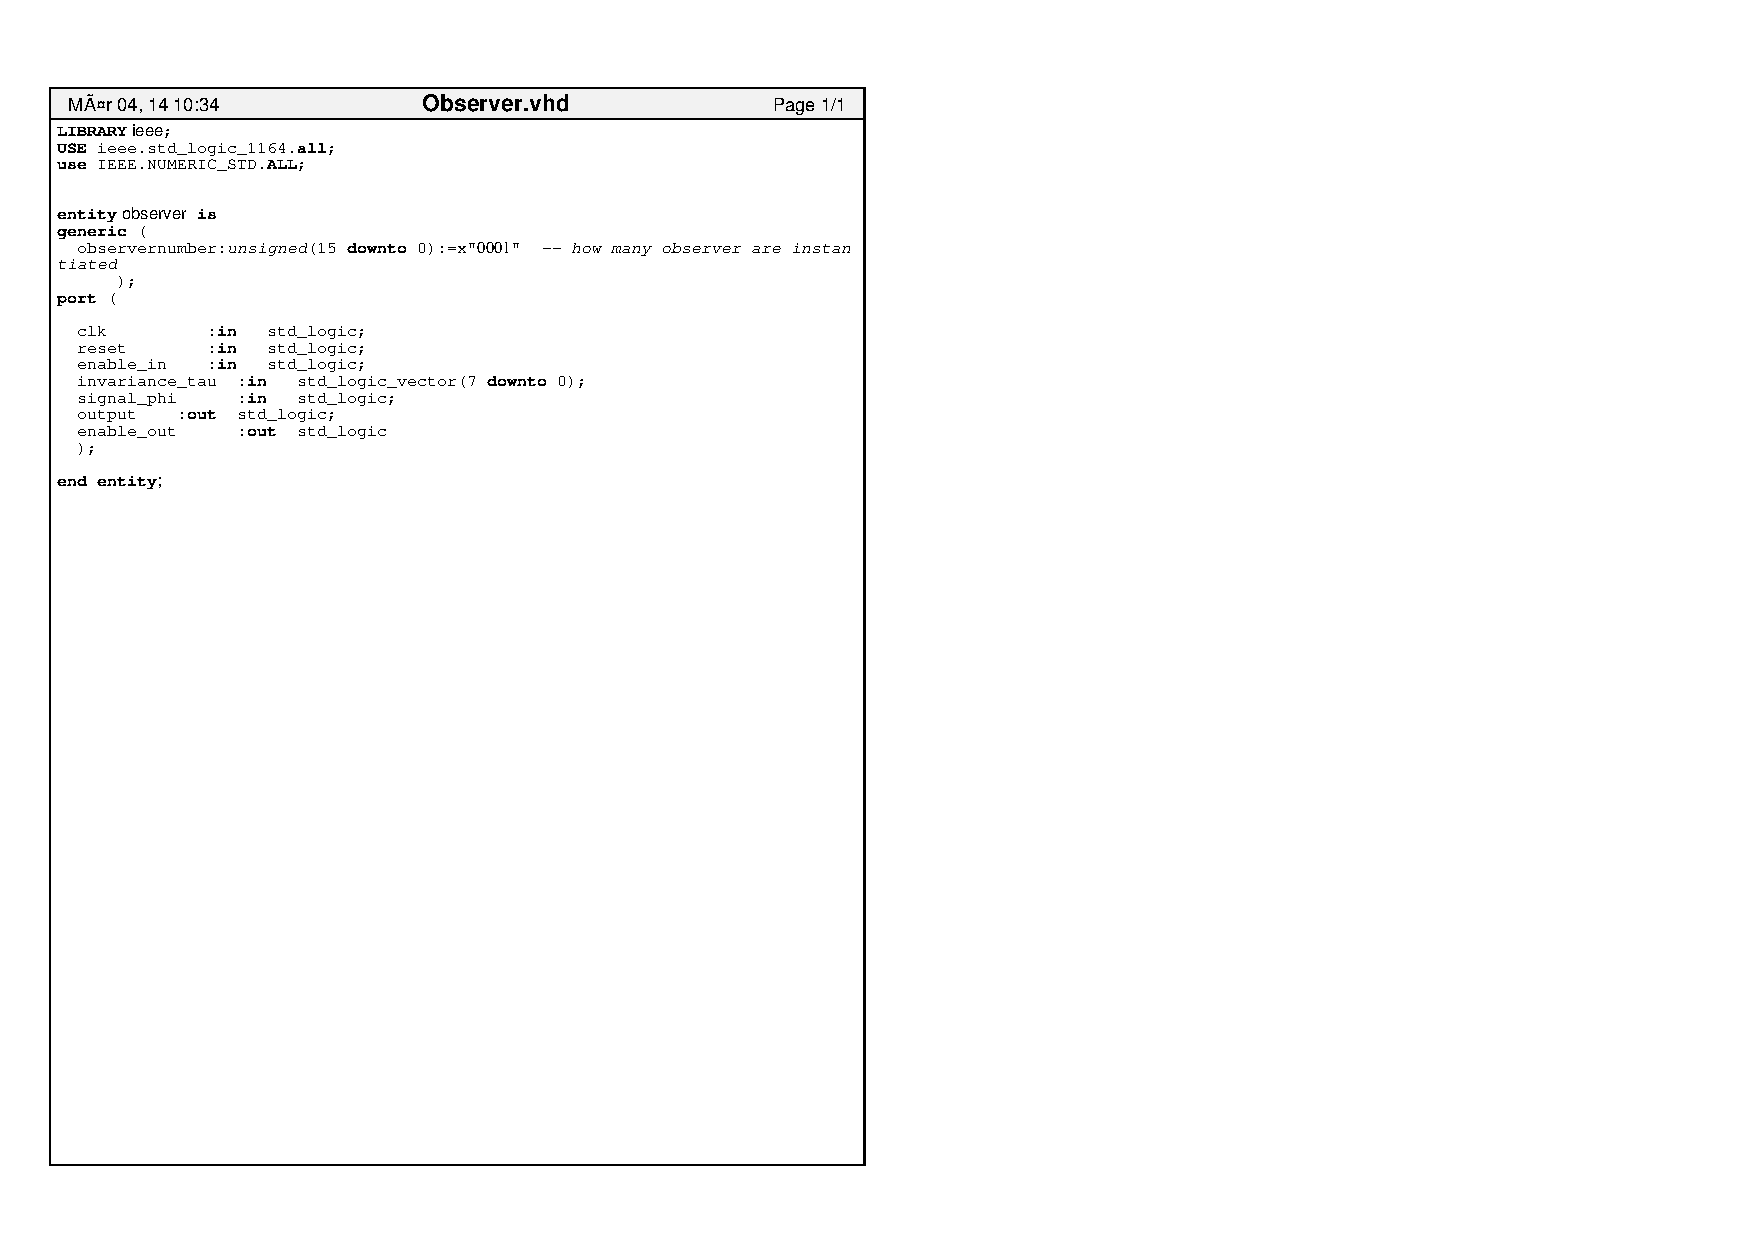
\includepdf[
 pages={-},
 nup=1x1,
 %landscape=false,
 %fitpaper=true,
 %noautoscale=false,
 turn=false,
 scale=1.6, 
 %trim= 0mm 0mm 0mm 0mm,
 clip=true,
 pagecommand={},
 %delta=0mm 0mm
 offset=-80mm 0mm
]{Appendix1/pdf/Observer.pdf}
\label{appendix:source:2}
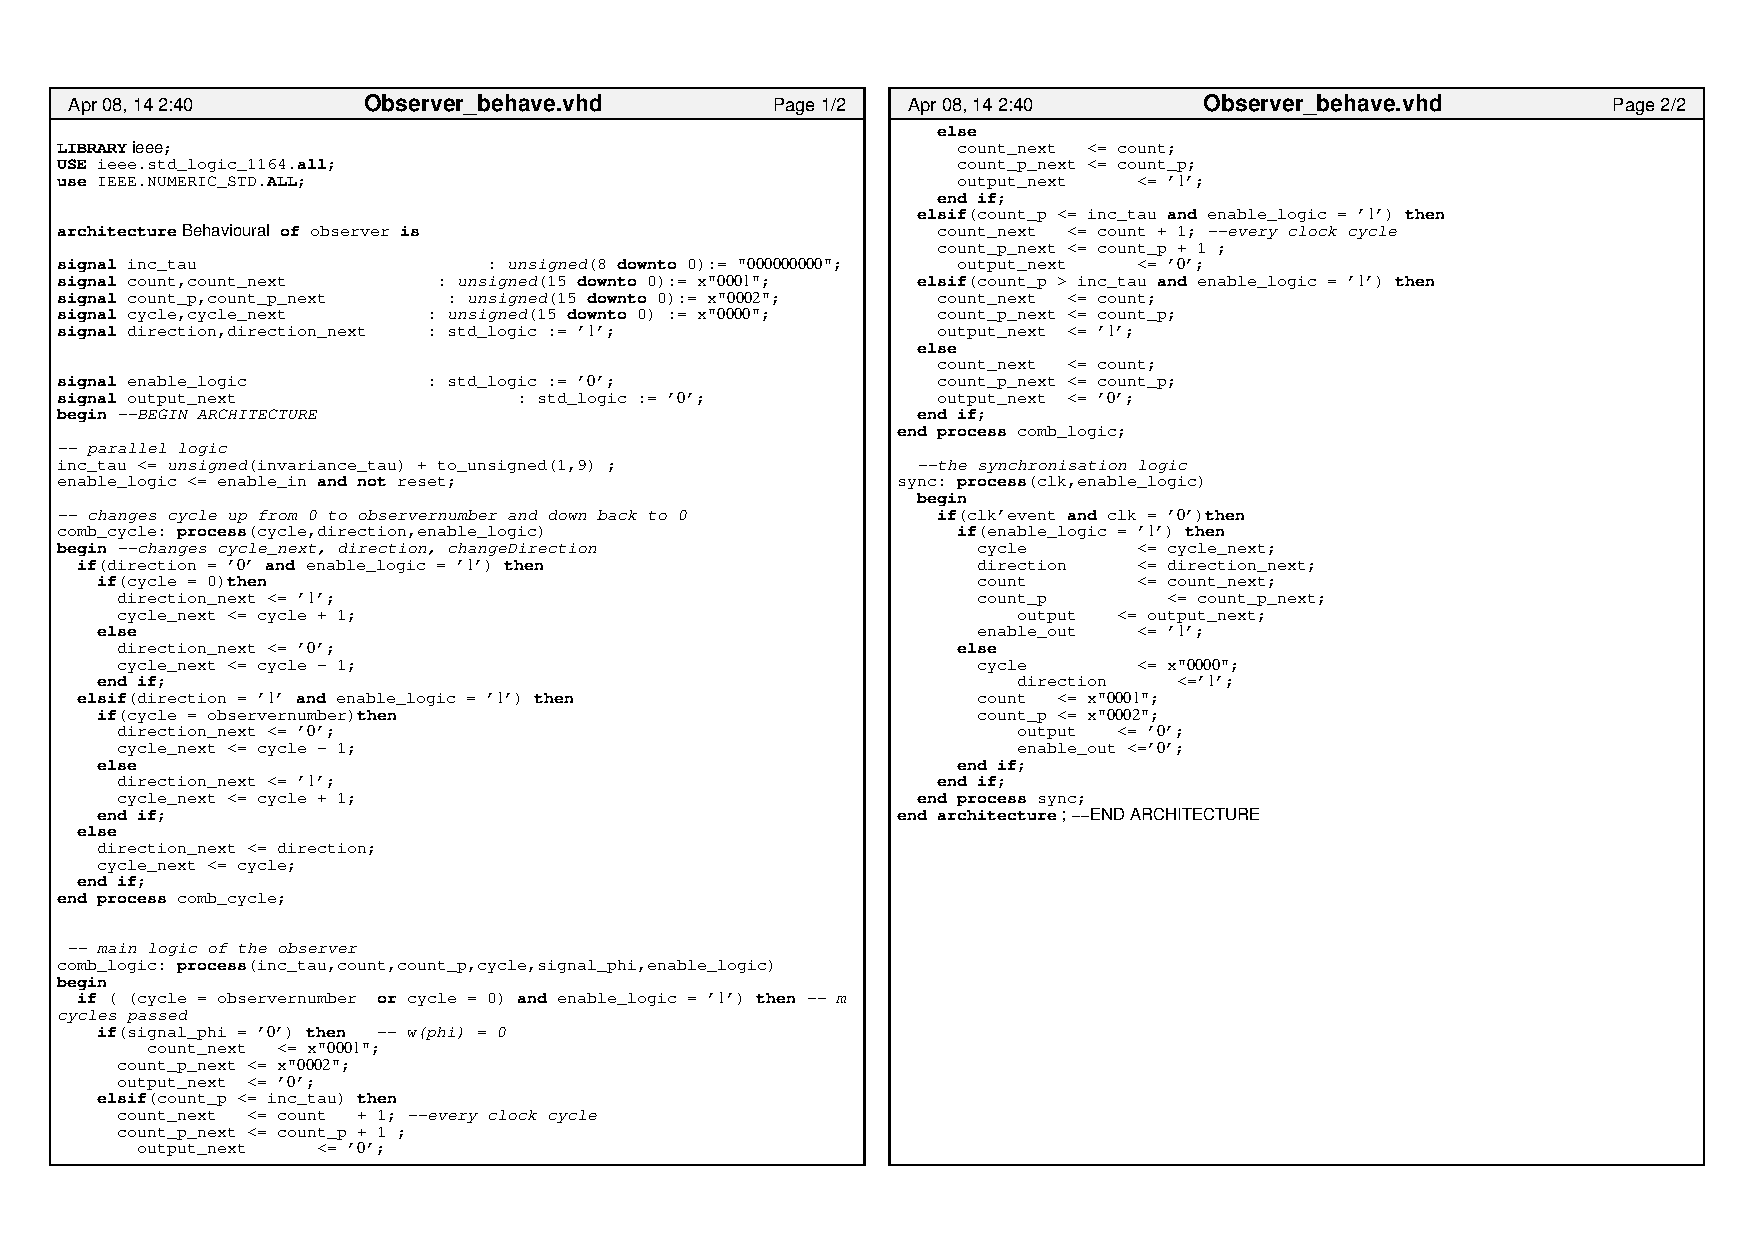
\includepdf[
 pages={-},
 nup=1x1,
 landscape=true,
 %fitpaper=true,
 noautoscale=false,
 turn=false,
 scale=0.9,
 %trim= 0mm 0mm 0mm 0mm,
 clip=true,
 pagecommand={},
 %delta=0mm 0mm
 %offset=-80mm 0mm
]{Appendix1/pdf/Observer_behave.pdf}
